\section{Evaluation}
In the following chapter the mobile implication of \enquote{\gls{see}} will be evaluated in a user study.
Therefore, the mobile application will be compared with the desktop version.

This chapter will start with a description of the desktop version and its main differences in section \ref{desktop}. 
Continuing with a defined aim and the precise hypotheses for the user study in section \ref{aim}.
After sketching the first experiment set up in section \ref{experiment} the actual experiment set up will be discussed in detail in section \ref{real} including the used survey tool, questionnaires and the pilot study.
\subsection{"SEE" Desktop}
\label{desktop}
In this section the desktop version of \enquote{\gls{see}} will be explained. 
In this evaluation the mobile version of \enquote{\gls{see}} will be compared with the desktop version.
Therefore, it is necessary to take a deeper look at the differences between those two versions.
Especially at how the interactions differ and what impact it could have on the user experience.

One outstanding difference from the desktop version to the mobile version is the selection of the interaction modes.
While in the mobile version the menu for the interaction modes is always visible in the desktop version by pressing space a menu screen opens as seen in figure \ref{fig:menu}.
Alternatively interaction modes can be changed by pressing one of the "1-9" keys, which, however requires the user to memorize which number belongs to which mode.

Another difference is the type of user input.
The desktop version uses mouse hovering to display the name of a hovered \enquote{\gls{node}} or \enquote{\gls{plane}}.
\begin{figure}[htb]
  \centering
  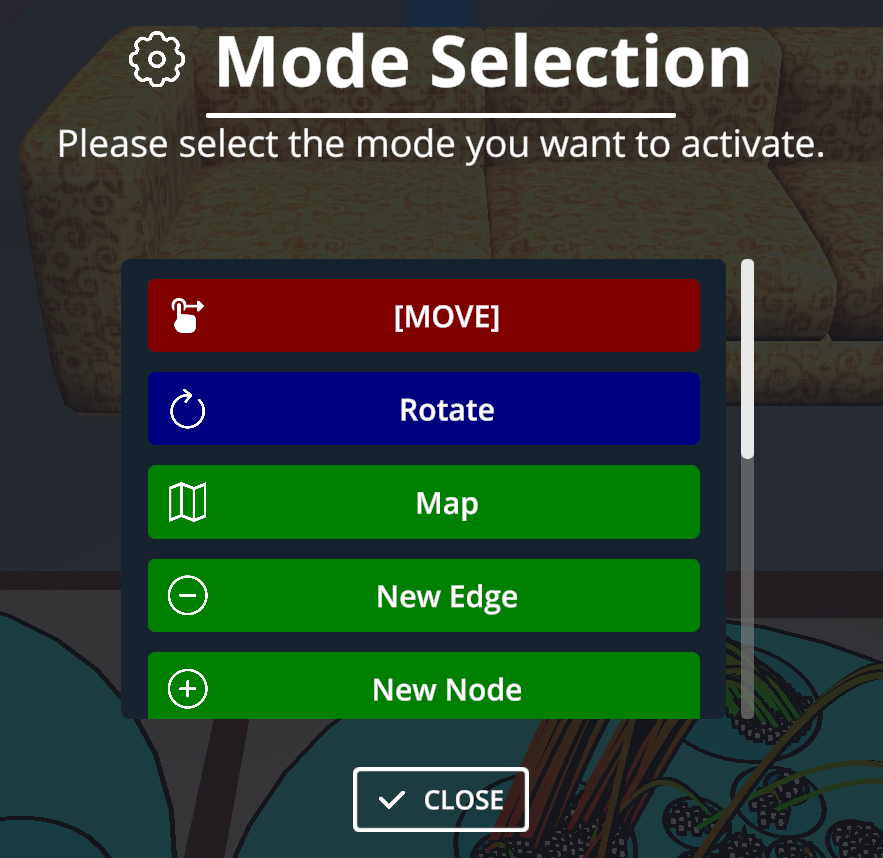
\includegraphics[width=0.8\textwidth]{Evaluation/img/menu.png}
  \caption{The desktop menu for selecting interaction modes.}\label{fig:menu}
\end{figure}
\subsection{Aim and hypothesis}
\label{aim}
The finished prototype of the mobile extension shall be evaluated. 
Therefore, the system shall be compared on smartphones as well as desktop computers. 
Comparing these two use cases shall give insight on how much impact the constraints of mobile devices have on the usability and overall user experience.

The hypotheses of this thesis is that the mobile version of \enquote{\gls{see}} lacks slightly in usability compared to the desktop version.
This due to the constraints of the mobile device. 
A smartphone has far less screen space and also does not have a physical keyboard, which would allow many more shortcuts.
\subsection{Experiment set up}
\label{experiment}
The system shall be tested in two groups each starting with a different device. 
Each group does the test on both devices, but one group will start with the mobile application and the other one with the desktop application.
The participants will be assigned random to the groups.
The testers will have various tasks to test the usability of the two applications. 
Afterwards the users will get a survey in English to document their impressions.
\begin{figure}[htb]
  \centering
  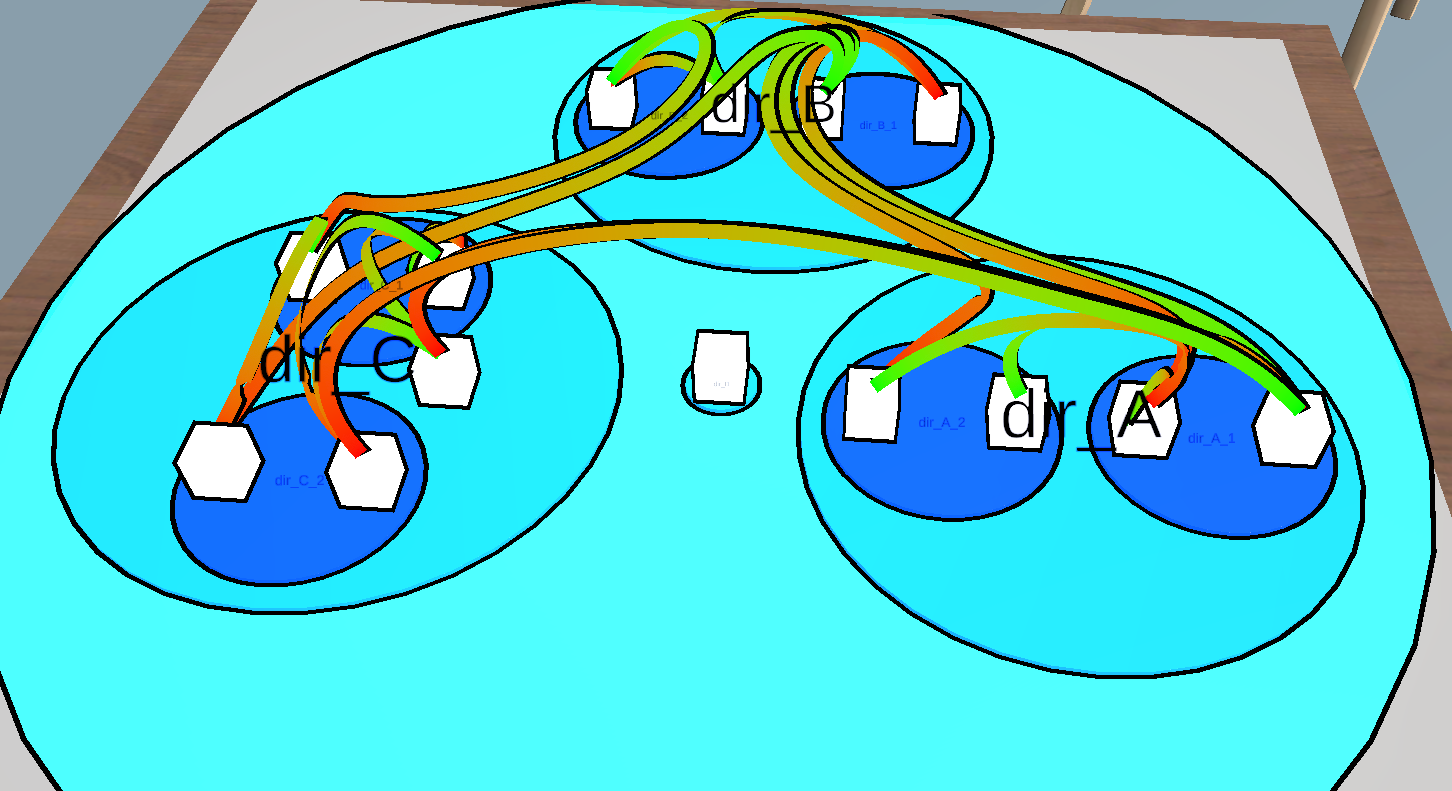
\includegraphics[width=1\textwidth]{Evaluation/img/city_1.png}
  \caption{The first \enquote{\gls{city}} for the user study}\label{fig:city1}
\end{figure}

\begin{figure}[htb]
  \centering
  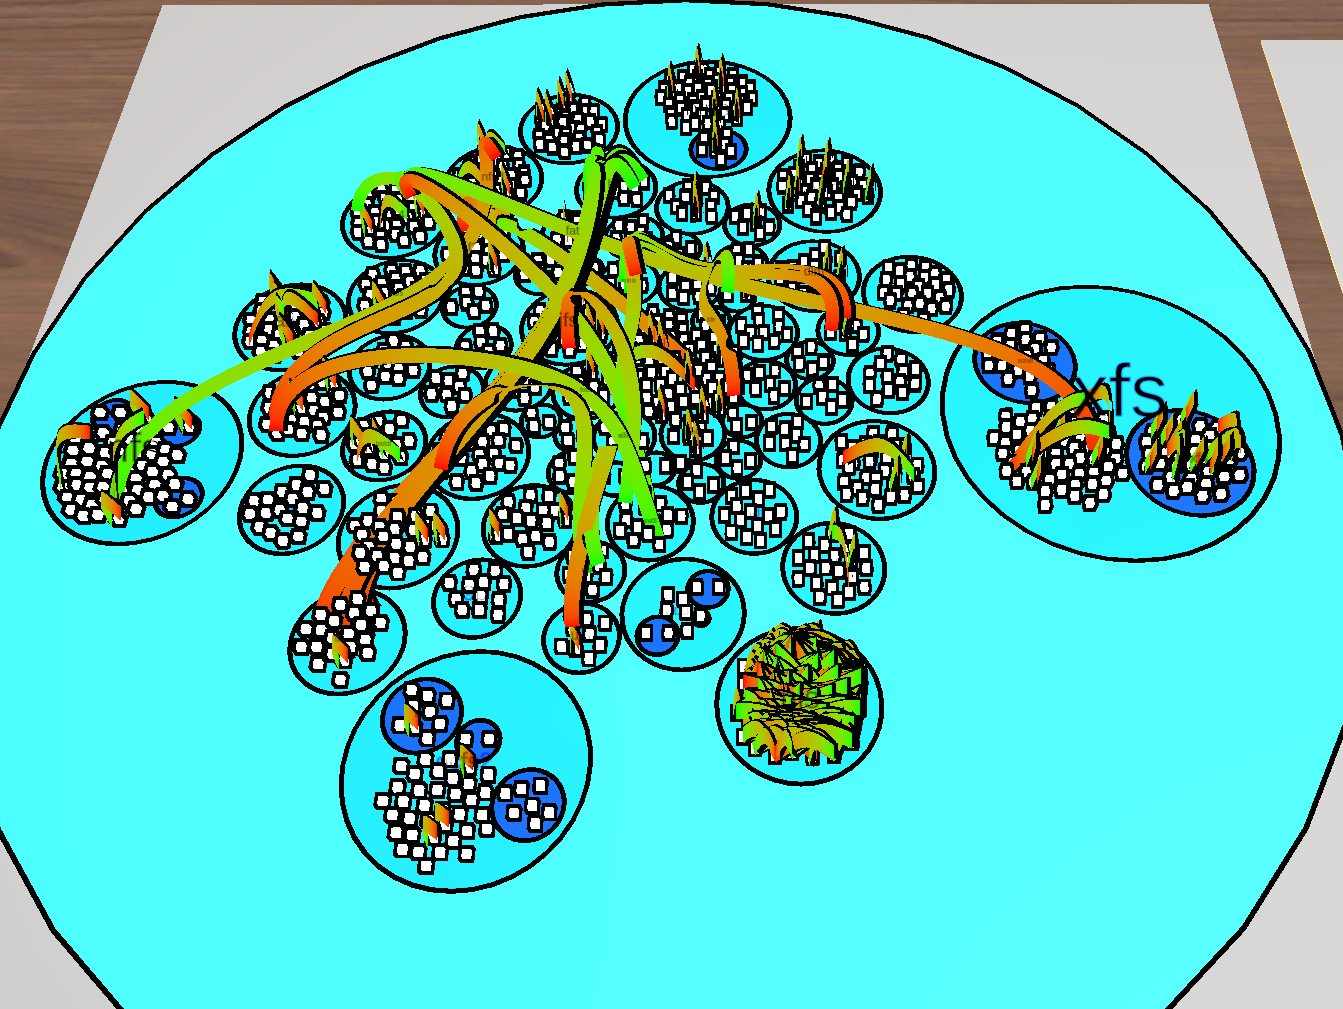
\includegraphics[width=1\textwidth]{Evaluation/img/city_2.png}
  \caption{The second \enquote{\gls{city}} for the user study}\label{fig:city2}
\end{figure}

\begin{figure}[htb]
  \centering
  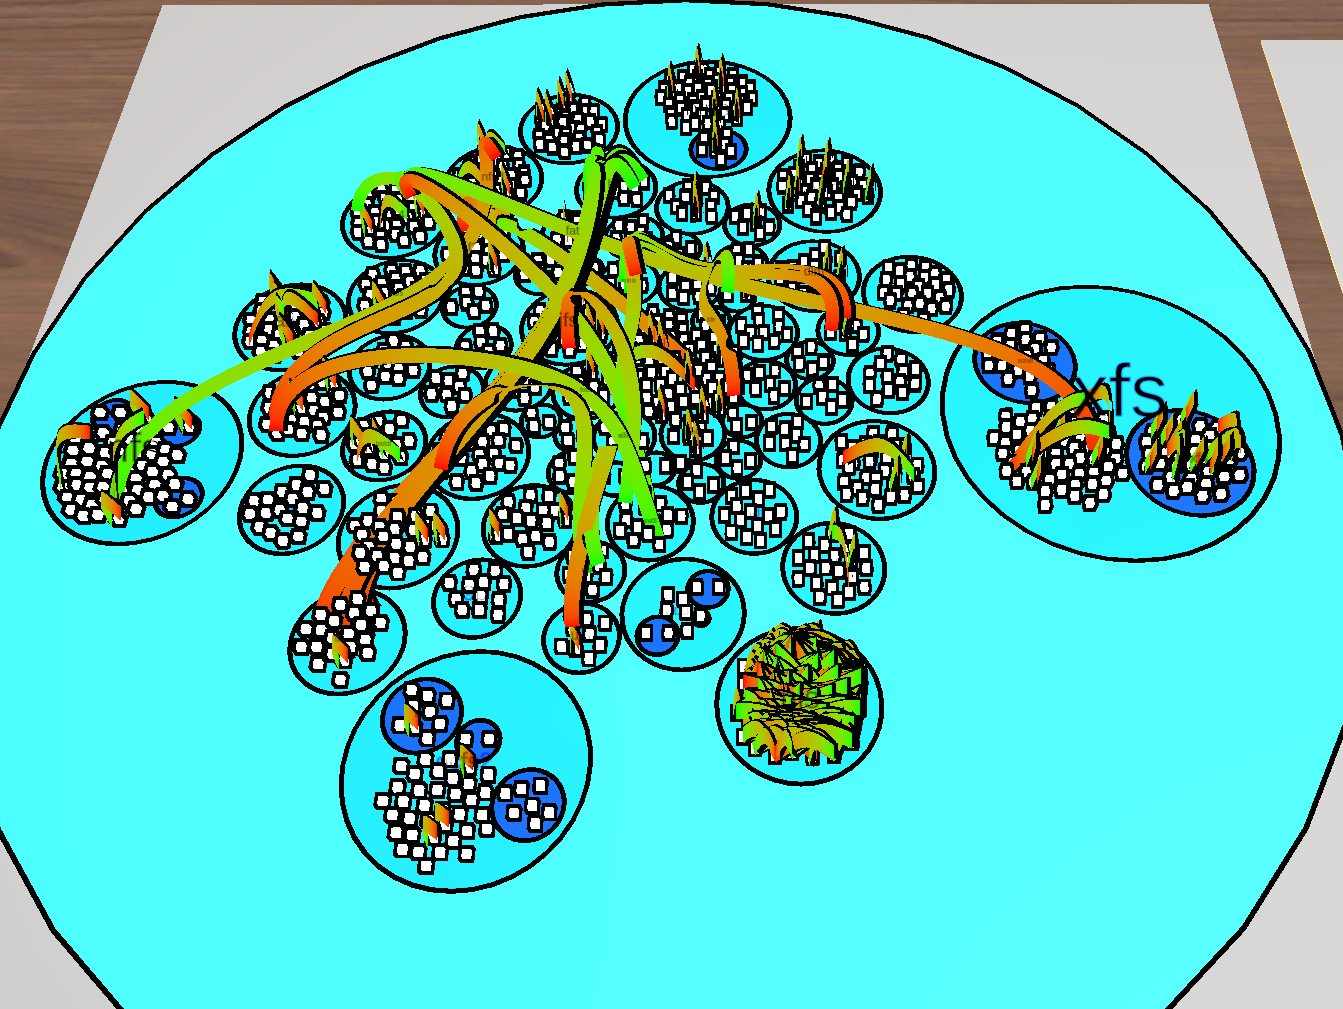
\includegraphics[width=1\textwidth]{Evaluation/img/city_3.png}
  \caption{The third \enquote{\gls{city}} for the user study}\label{fig:city3}
\end{figure}
In this survey the subjects will be asked various demographic questions as well as what Android device and version they will be using.
In addition to that the subjects will be asked if they are experienced with \enquote{\gls{see}} and if they are experienced with software development.
Before the subjects will be asked to solve various tasks they will be asked to watch a short tutorial video on each application.
After the video they will get a training task where every subject can get used to the system and ask questions if they have trouble solving the training task. 
The overseer will also make sure that every essential action will be practiced such as zooming and moving the \enquote{\gls{city}}.
Figure \ref{fig:city1} shows a small arranged \enquote{\gls{city}} that shall be used for the training tasks.
The structure of the training \enquote{\gls{city}} is generic and follows a simple pattern. 
That shall ensure that the user can focus on the training and that the user does not get overwhelmed. 

Following the first questions and the training, the subjects can start with the main tasks.
For each application there will be two tasks and after each task the subjects will be handed a \enquote{\gls{post-task}} questionnaire.
Last but not least there will another questionnaire that aims to scale the \enquote{\gls{usability}} of the two applications.
For the \enquote{\gls{post-task}} questions the \enquote{\gls{ASQ}} will be used and for the \enquote{\gls{usability}} questions \enquote{\gls{sus}} will be used.
Both questionnaires will be discussed later on in section \ref{questionaires}.
For each main task the overseer will also take the completion time of every main task.
The first and second task on the first device will be performed on the \enquote{\gls{city}} that can be seen in figure \ref{fig:city2} and the third and forth task on device two will be performed on the \enquote{\gls{city}} that can be seen on figure \ref{fig:city3}.
These examples are much larger than the training \enquote{\gls{city}} and represent real life code.
The second \enquote{\gls{city}} shows the file system of Linux and the third one shows the network component of Linux. 
That way the tasks might reflect better on real world uses for \enquote{\gls{see}}.

To not exhaust the testers too much the experiment shall not take longer than one hour. 
This also ensures that there is no to little variance due to exhaustion.
Each participant might have a different concentration span, but this shall not be the focus of this experiment. 

\subsection{Realization}
\label{real}
\subsubsection{Survey tool}
\subsubsection{Questionnaires}
\label{questionaires}
\subsubsection{Pilot study}
In a first test the pilot study was executed with one tester. 
Afterwards the study was discussed and checked for errors. 
It stood out that the example \enquote{\gls{city}} of task one was too different to the one in the second task.
Therefore, the \enquote{\gls{city}} of the first task was exchanged with a larger and better comparable one.
Further on a \enquote{\gls{city}} with 1288 nodes (see figure \ref{fig:city2}) as well as one with 1464 nodes (see figure \ref{fig:city3}) will be used.

Also, the tasks were not comparable because they differed in the types of interactions they used.
In one task the user was asked to rename a node and in the other one the user shall add four nodes.
For renaming a node the user has to use a keyboard which does not make it comparable to just click and add nodes in the second task.




\begin{figure}[htb]
    \centering
    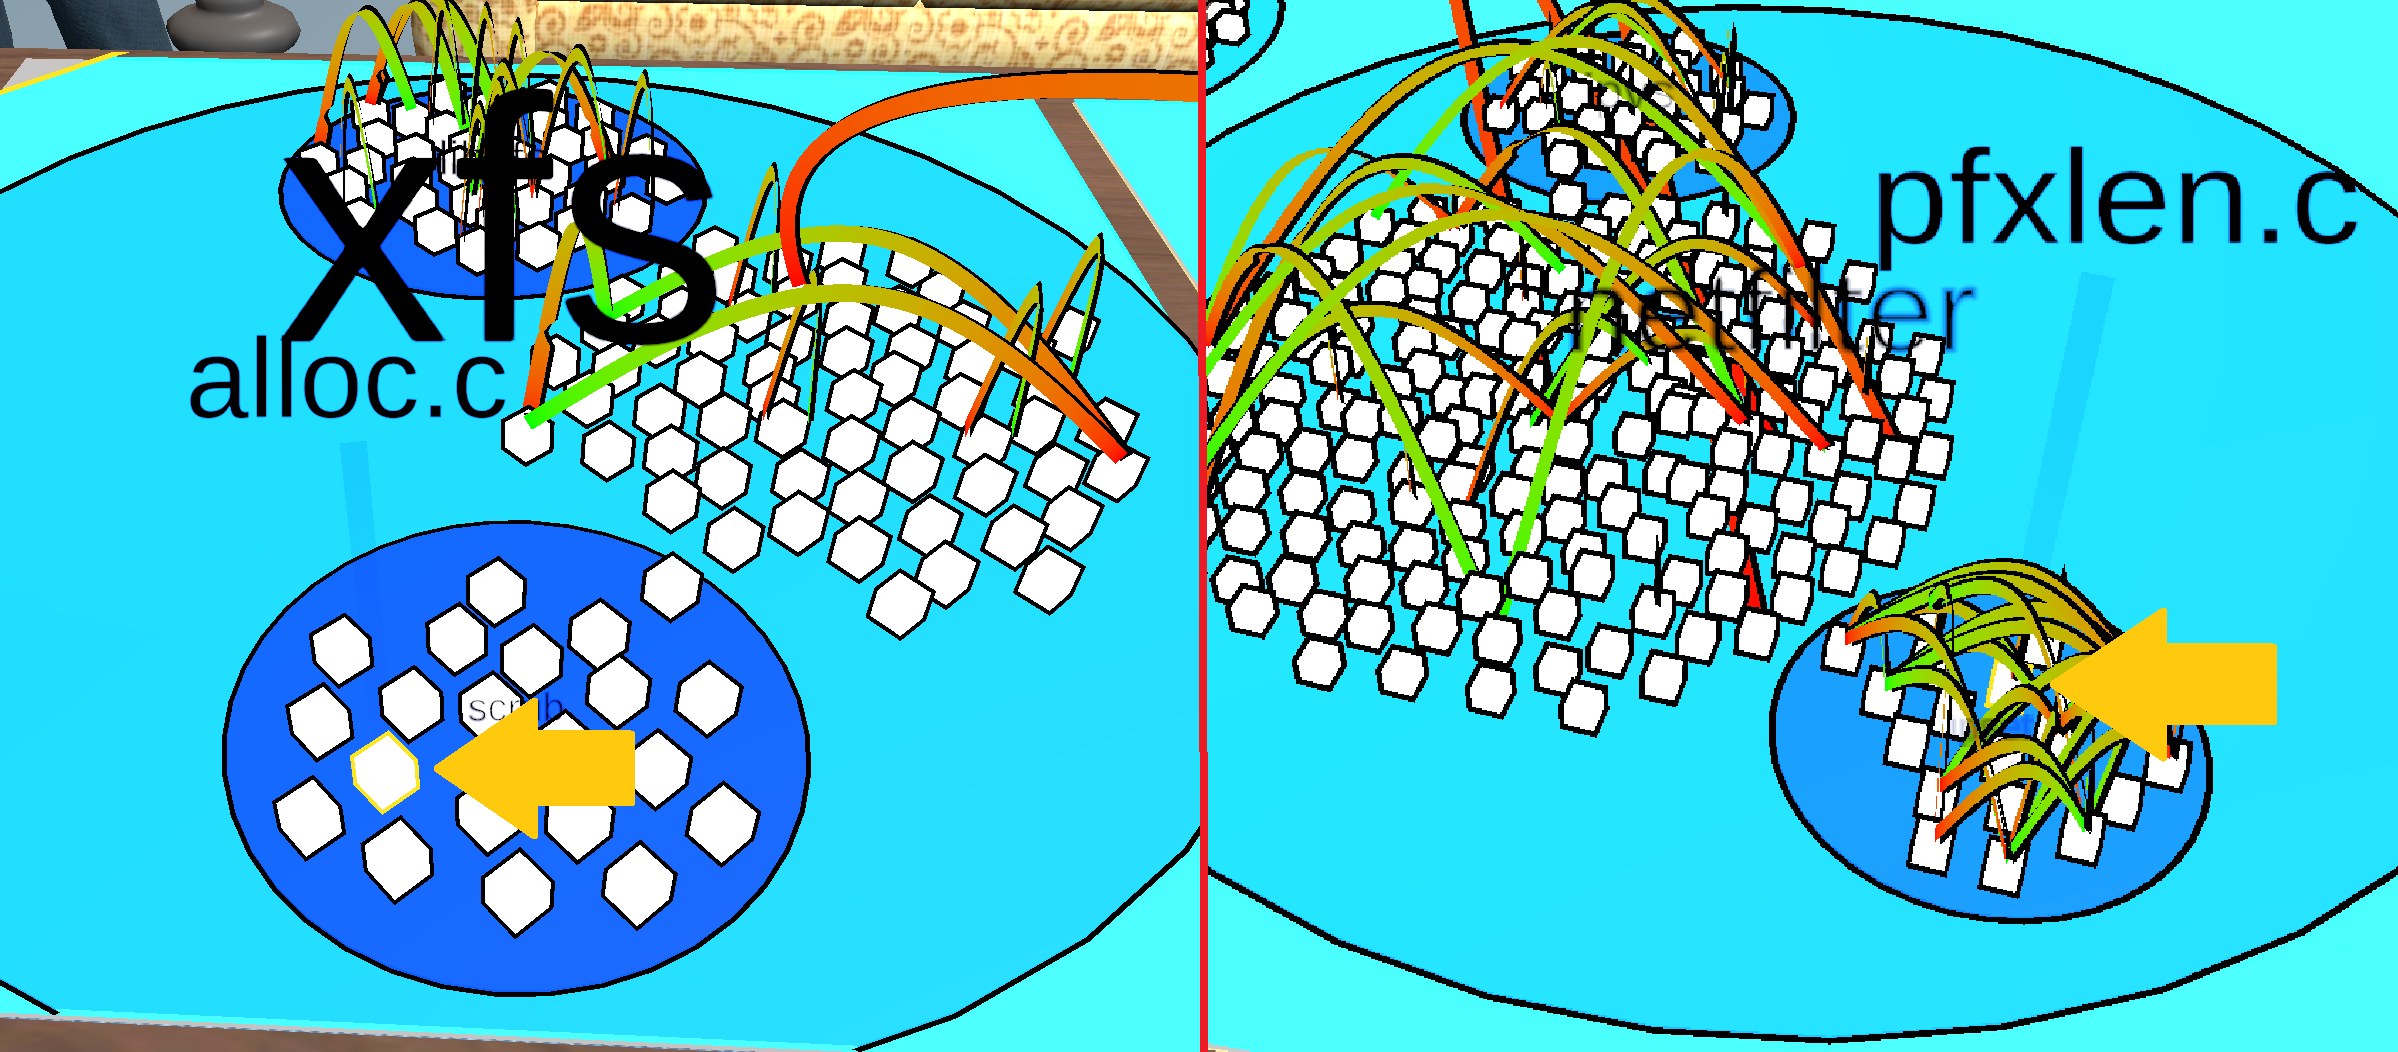
\includegraphics[width=1\textwidth]{Evaluation/img/task1.png}
    \caption{The two key nodes are marked with a yellow arrow}\label{fig:task1}
\end{figure}

\subsubsection{Final experiment set up}

Demographic questions:
\begin{itemize}
    \item Age
    \begin{itemize}
        \item 0-15 years old
        \item 16-30 years old
        \item 31-45 years old
        \item 46+ years old
    \end{itemize}
    \item What gender do you identify as?
    \begin{itemize}
        \item Male
        \item Female
        \item Other ...
        \item Prefer not to say
    \end{itemize}
    \item What is the highest degree or level of education you have completed?
    \begin{itemize}
        \item Some High School (Hauptschule/Realschule...)
        \item High School (Abitur)
        \item Bachelor's Degree
        \item Master's Degree
        \item Ph.D. or higher
        \item Prefer not to say
        \item Other ...
    \end{itemize}
\end{itemize}

Questions regarding used hardware and experience
\begin{itemize}
    \item Are you already experienced with See? 
    \item Do or did you play first person video games?
    \item Do or did you develop software? 
    \item On which Android device will you attend?
    \item Which Android version are you using?*
\end{itemize}

\begin{table}[]
    \resizebox{\textwidth}{!}{%
    \begin{tabular}{lll}
    Nr. &
      Task &
      Expected time \\ \hline
    Training &
      \begin{tabular}[c]{@{}l@{}}Navigate through the planes "dir\_root" \\ \textgreater "dir\_B" \textgreater "dir\_B\_2". On that plane \\ select "b2\_b.cpp" and rename it "b42".\end{tabular} &
      1 - 5 mins \\
    1 &
      \begin{tabular}[c]{@{}l@{}}Detect the largest plane "xfs". On that\\ plane find plane "scrub". Then find \\ and delete node "alloc.c".\end{tabular} &
      0.5 - 5 mins \\
    2 &
      \begin{tabular}[c]{@{}l@{}}Find the plane with one blue child \\ plane ("btrfs"). On the blue child \\ plane "tests" add four new nodes.\end{tabular} &
      1 - 5 mins \\ \hline
    Training &
      \begin{tabular}[c]{@{}l@{}}Navigate through the planes "dir\_root" \\ \textgreater "dir\_C" \textgreater "dir\_C\_2". On that plane \\ select "c2\_b.cpp" and rename it "c42".\end{tabular} &
      1 - 5 mins \\
    3 &
      \begin{tabular}[c]{@{}l@{}}Detect the \\ largest plane "netfilter". On that plane\\ find plane "ipset". Then find and \\ delete node "pfxlen.c".\end{tabular} &
      0.5 - 5 mins \\
    4 &
      \begin{tabular}[c]{@{}l@{}}On the plane with the most \\ edges ("ipv6") find the smallest plane\\ "ila" and connect all four nodes on it.\end{tabular} &
      1 - 5 mins \\ \hline
    \end{tabular}%
    }
    \caption{The tasks used for the experiment. The device will be switched after task 2.}
    \label{table:tasks}
    \end{table}
    
\begin{table}[]
    \resizebox{\textwidth}{!}{%
    \begin{tabular}{llll}
    Phase          &      & \multicolumn{2}{l}{Description}                     \\ \hline
    Pre-Experiment &      & \multicolumn{2}{l}{Demographic questionnaire}       \\ \hline
                   & City & Group 1                  & Group 2                  \\ \hline
    Training       & Figure \ref{fig:city1}   & \multirow{6}{*}{Desktop} & \multirow{6}{*}{Mobile}  \\
    Task 1         & Figure \ref{fig:city2}    &                          &                          \\
    ASQ            &      &                          &                          \\
    Task 2         & Figure \ref{fig:city2}    &                          &                          \\
    ASQ            &      &                          &                          \\
    SUS            &      &                          &                          \\ \hline
    Training       & Figure \ref{fig:city1}   & \multirow{6}{*}{Mobile}  & \multirow{6}{*}{Desktop} \\
    Task 3         & Figure \ref{fig:city3}   &                          &                          \\
    ASQ            &      &                          &                          \\
    Task 4         & Figure \ref{fig:city3}    &                          &                          \\
    ASQ            &      &                          &                          \\
    SUS            &      &                          &                         
    \end{tabular}%
    }
    \caption{Experimental procedure per subject. The procedure is swapped per group.}
    \label{table:procedure}
    \end{table}


\subsubsection{Execution}